\documentclass{article}
\usepackage{mathtools}
\usepackage[top=2in, bottom=1.5in, left=1in, right=1in]{geometry}
\usepackage{graphicx}
\usepackage[normalem]{ulem}
\usepackage{fancyhdr}
\usepackage{enumerate}
\pagestyle{fancyplain}

\lhead{PHYS 152 Section 10}

\rhead{A. Shawn Bandy 
(003635396)}

\begin{document}
\title{Lab \#4:  Basic Electric Circuits \& Measurements}
\author{A. Shawn Bandy}
\date{February 25, 2013}
\maketitle
\begin{abstract}
In this lab we applied electrical energy to two circuits:  one with an {\it{unknown}} resistor and one with a small lightbulb acting as a resistor.  Using a variable resistance box and an electric generator, we measured the volts and current using a digital multimeter and a handheld digital multimeter.  This data was then used to produce I-V curve graphs and estimates for R that we compared to director measurement.
\end{abstract}
\section{Data and Data Tables}

\begin{description}

\item[DATA SHEET \#1] \hfill
\begin{description}
Direct ohmmeer readings of resistance ($\Omega$) from the DMM:\
\item[1. For the resistor R:] R = 32.8 $\Omega$  \
\item[2. For the light bulb (approximately at room temperature before applying voltage)] R = 5.7 $\Omega$  \\
\end{description}
\begin{samepage}
\textbf{ TABLE 2.1 Measurements of V and I for the unknown resistance R. } \
{\small{
\begin{center}
	\begin{tabular}{| l | l | l | l | l | l | l |}
	\hline
	&V (mV) & I (mA) & & V (mV) & I (mA) \\ \hline
	1	&4.73	&146.8	&11	&3.57	&110.9 \\ \hline
	2	&4.62	&143.4	&12	&3.45	&107.3 \\ \hline
	3	&4.53	&140.9	&13	&3.35	&103.9 \\ \hline
	4	&4.46	&138.2	&14	&3.21	&99.7 \\ \hline
	5	&4.36	&135.4	&15	&3.02	&93.5 \\ \hline
	6	&4.28	&132.8	&16	&2.93	&91 \\ \hline
	7	&3.93	&122.4	&17	&2.82	&87.8 \\ \hline
	8	&3.85	&119.4	&18	&2.72	&84.8 \\ \hline
	9	&3.72	&115.4	&19	&2.62	&81.3 \\ \hline
	10	&4.08	&125.6	&20	&3.11	&96.8 \\ \hline
	\end{tabular}
\end{center}
}}
\end{samepage}
\begin{samepage}
\textbf{ TABLE 2.2 Measurements of V and I for the resistance of the light bulb. } \
{\small{
\begin{center}
	\begin{tabular}{| l | l | l | l | l | l | l | l | l |}
	\hline
	&V (mV) & I (mA) & $R = \frac{V}{I}(\Omega)$ & & V (mV) & I (mA) & $R = \frac{V}{I}(\Omega)$  \\ \hline
	1	&2.14	&	63.1	&	0.0339144216	&11	&	0.93	&	42	&	0.0221428571 \\ \hline
	2	&2.07	&	62.3	&	0.0332263242	&12	&	0.79	&	39	&	0.0202564103 \\ \hline
	3	&1.86	&	60	&	0.031		&13	&	0.68	&	37.1	&	0.018328841\\ \hline
	4	&1.85	&	59	&	0.0313559322	&14	&	0.62	&	36	&	0.0172222222\\ \hline
	5	&1.74	&	57	&	0.0305263158	&15	&	0.58	&	34.9	&	0.0166189112\\ \hline
	6	&1.62	&	54.6	&	0.0296703297	&16	&	0.45	&	32.8	&	0.0137195122\\ \hline
	7	&1.41	&	51.5	&	0.0273786408	&17	&	0.34	&	31	&	0.0109677419\\ \hline	
	8	&1.23	&	48.2	&	0.0255186722	&18	&	0.33	&	30.4	&	0.0108552632\\ \hline
	9	&1.16	&	46.5	&	0.0249462366	&19	&	0.25	&	28.1	&	0.0088967972\\ \hline
	10	&1.05	&	44.5	&	0.0235955056	&20	&	0.19	&	25.9	&	0.0073359073\\ \hline

	\end{tabular}
\end{center}
}}
\end{samepage}
\item[DATA SHEET \#2] \hfill
\begin{description}
\item[A.] See Graphs.
\item[B.] See Graphs.  Slope was determined by ordinary least squares, one variable by mathematica.  Slope = $\frac{cov(current,voltage)}{var(voltage)} $
\item[C. Comparison of experimental and directly measured values for the resistor R]\
\begin{description}
\item[Value of R from graph: ] R = 30.9349 $\Omega$\
\item[Value of R from direct measurement: ] R = 32.8 $\Omega$\
\item[Percent Difference: ] $|\frac{R_{GRAPH} - R_{DMM}}{R_{DMM}}|$ = 0.05682\
\end{description}
\end{description}
\item[DATA SHEET \#3] \hfill \\
{\it{See Answers to Questions}}
\end{description}
\section{Graphs}\hfill\\
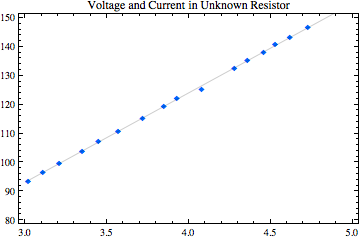
\includegraphics{lab4_graph_1}\\

{\tiny{
\begin{verbatim}
Mathematica:
volts = {4.73, 4.62, 4.53, 4.46, 4.36, 4.28, 3.93, 3.85, 3.72, 4.08, 
   3.57, 3.45, 3.35, 3.21, 3.02, 2.93, 2.82, 2.72, 2.62, 3.11};
current = {146.8, 143.4, 140.9, 138.2, 135.4, 132.8, 122.4, 119.4, 
   115.4, 125.6, 110.9, 107.3, 103.9, 99.7, 93.5, 91, 87.8, 84.8, 
   81.3, 96.8};
data = Table[{volts[[i]], current[[i]]}, {i, Length[volts]}];
reg = FindFit[data, a + b x, {a, b}, x];
Show[
 ListPlot[{{{80, 150}}, {{3, 5}}, data}, 
  PlotMarkers -> {Automatic, Small}, PlotStyle -> Hue[0.6], 
  Axes -> True],
 Plot[ (a + b x) /. reg, {x, 3, 5}, PlotStyle -> {GrayLevel[0], Thin}],
 PlotRange -> {{3, 5}, {80, 150}},
 Frame -> True,
 Axes -> True,
 PlotLabel -> "Voltage and Current in Unknown Resistor"
\end{verbatim} 
}}
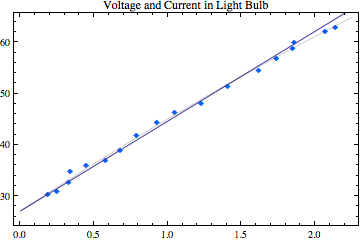
\includegraphics{lab4_graph_2}\\
Note:  Directly measured resistance is darker line (slope = 17.54, intercept = 27.1079)
{\tiny{
\begin{verbatim}
Mathematica:
volts = {2.14, 2.07, 1.86, 1.85, 1.74, 1.62, 1.41, 1.23, 1.05, 0.93, 
   0.79, 0.68, 0.58, 0.45, 0.34, 0.33, 0.25, 0.19};
current = {63.1, 62.3, 60, 59, 57, 54.6, 51.5, 48.2, 46.5, 44.5, 42, 
   39, 37.1, 36, 34.9, 32.8, 31, 30.4, 28.1, 25.9};
data = Table[{volts[[i]], current[[i]]}, {i, Length[volts]}];
reg = FindFit[data, a + b x + c x^2, {a, b, c}, x];

Show[
 
 ListPlot[{{{25, 65}}, {{0, 2.25}}, data}, 
  PlotMarkers -> {Automatic, Small}, PlotStyle -> Hue[0.6], 
  Axes -> True],
 Plot[17.54 x + 27.1079, {x, 0, 2.25}],
 Plot[ (a + b x + c x ^2) /. reg, {x, 0, 2.25}, 
  PlotStyle -> {GrayLevel[0], Thin}],
 PlotRange -> {{0, 2.25}, {25, 65}},
 Frame -> True,
 Axes -> True,
 PlotLabel -> "Voltage and Current in Light Bulb"
 ]
\end{verbatim} 
}}
\section{Results}\hfill\\
The direct measure for the resistor was 32.8 $\Omega$ vs 39.9349 
 $\Omega$ (mean value of samples). \\
The measurement error for the resistance of the resistor was 0.05682 or about 5.7\%.\\
The direct measure for the resistance of the light bulb filiament was 5.7 $\Omega$.  The fitted quadratic for these measurements had the following coefficients ($a+bx+cx^2$): a = 27.1079, b= 18.9085, c = -0.935176.
\section{Discussion}\hfill\\
We began by measuring the resistance of the resistor and the light bulb with the digital multimeter.  Next we constructed the circuit as described in the lab procedure.  Two digital multimeters (DMM) were used to measure the voltage and current in the circuit when the DC power supply was active.  One measured the voltage potential on each side of the resistor/light bulb.  The other was in series in the circuit between the variable resistor device and the power supply.  \\ \\
At times, the circuit seemed to be sensitive to touch or vibration.  Some uncertainty in our measurements simply arise because the act of, say, changing the resistance value on the box may have altered the measurement by some unknown amount.  A second source of error may have been in the variable resistor box itself.  Changing the setting and then changing back would yield slightly different readings on the DMMs.  When measuring the light bulb and especially at higher resistance values on the variable resistor box, we observed what appeared to be oscillating values on the DMM.  We do not know if this phenemenon is a feature of the variable resistance of the light bulb or because as the value for the current is decreases the value for R is more sensitive to changes in I because $R=\frac{V}{I}$.  Never the less, the overall error - the difference between directly and indirectly calculated resistance - is reasonably small for the scope of this lab procedure.
\section{Answers to Questions}\hfill\\
\begin{description}
\item[A.] What causes electric resistance in materials? \hfill\\
Electrical resistance is the resistance to the flow of electrons through a material, in some sense similar to friction.  
\item[B.] State Ohm's law using words. \hfill\\
The current flowing through a material at two point varies directly with with the voltage difference between those two points.  The coefficient is electrical resistance.  Hence $V = \frac{I}{R}$.
\item[C.] This question refers to the V versus I plot for the light bulb.  Can this nonlinear-resistance device be made to seem linear by restricting the range of voltages or currents used?  HINT: look near the origin of the graph. \hfill\\\\
As $\Delta$V approaches zero, resistance approaches the slope of the tangent of the V/I curve.
\end{description}
\end{document}